\textbf{The Infamous Runge-Phenomenon} It is not generally true that higher degree interpolation polynomials yield more accurate approximations. Let $$ f(x) = \frac{1}{1 + x^2} \text{ and } x_j = -5 +jh, j = 0, 1, \cdots, n, h = \frac{10}{n}.$$
For $$n = 1, 2, 3, \cdots, 20$$ plot the graph of the interpolant $$p(x) = \Sigma_{i = 0}^n \alpha_i x^i$$ defined by $p(x_i) = f(x_i).$

\textbf{Proof}\\
Below are the graphs of $f(x)$ and $p_{20}(x)$. You can see that interpolating along equally spaced intervals yields polynomials that oscillate wildly toward the final end points.

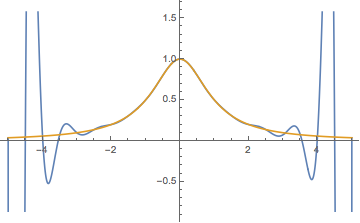
\includegraphics[scale = .5]{rungePhenomenon.png}

The plot is too cluttered with additional lines. However, the case where $n = 20$ is informative and shows the general issue with interpolating at equal intervals.